\documentclass{acmsiggraph}
\usepackage[scaled=.92]{helvet}
\usepackage{times}

\usepackage{rotating}
\newcommand{\rotxc}[1]{\begin{sideways}#1\end{sideways}}
\newcommand{\invert}[1]{\rotxc{\rotxc{#1}}}
\usepackage{graphicx}

%% use this for zero \parindent and non-zero \parskip, intelligently.

\usepackage{parskip}
\usepackage{footnote}

\renewcommand{\thefootnote}{\fnsymbol{footnote}}

\usepackage[labelfont=bf,textfont=it]{caption}
\usepackage{amsmath, amsthm, amssymb}

\newtheorem{thm}{Theorem}[section]
\newtheorem{cor}[thm]{Corollary}
\newtheorem{lem}[thm]{Lemma}

\theoremstyle{remark}
\newtheorem{rem}[thm]{Remark}

\theoremstyle{definition}
\newtheorem{defn}[thm]{Definition}

%Hacky pseudo-code:
\newcommand{\cF}[1]{{\tt #1}}
\newcommand{\cTAB}{\phantom{----}}
\newcommand{\cIF}{{\bf if}}
\newcommand{\cRET}{{\bf return}}
\newcommand{\cWHILE}{{\bf while}}
\newcommand{\cFOR}{{\bf for}}

\newcommand{\defbreak}{\vspace{1em}}
\title{The {\em fluint8} Software Integer Library}

\author{Jim McCann\thanks{e-mail: ix@tchow.com}\\TCHOW llc \and Your Name Here}

\teaser{
\centering
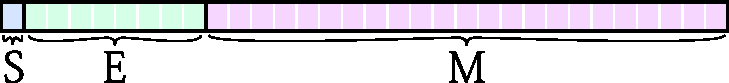
\includegraphics[width=3in]{ieee754-binary32.pdf} \huge $= -1^{S}\cdot 2^{E-127-23} \cdot (2^{23} + M)$
\caption{\label{fig-binary32}
Our library performs unsigned integer operations using only arithmatic operations on IEEE754 floating point numbers stored in binary32 format (pictured).
}}

%\keywords{anger, invective, morality}
\begin{document}

\maketitle

\begin{abstract}
We present {\em fluint8}, a library for performing integer math, including basic arithmetic and bitwise logical operations, using only basic floating point operations.
\end{abstract}

%D.2.3 = 0xD23 = 0x45523000 (floating point)
%         exponent:45
%0x305245
\begin{CRcatlist}
\CRcat{$(1.10100100011)_{2}\times{}2^{11}$}{Software}{Software Engineering}{\small Coding Tools and Techniques}
\end{CRcatlist}

\section{Introduction}
There are a surfeit of libraries that exist to perform floating point operations on processors that only support integer math.
This is unsurprising, as many such processors exist -- from ancient 286's to modern embedded microcontrollers.
These libraries use many integer instructions to emulate the action of a floating point unit, providing correct and useful (if slow) results.

We present a small header-only library to emulate integer operations -- specifically 8-bit unsigned integer operations -- using standard IEEE 754 single-precision (binary32) floating point math.
Our presented operations have been designed to be succinct but also pleasantly puzzling.

As far as we are aware, no processor exists for which this library would be required.
However, perhaps you should consider that a challenge.

\section{Floating Point}
An IEEE 754 single-precision floating point number (binary32 format) is stored as a sign bit, a 8-bit exponent, and a 23-bit mantissa (Figure~\ref{fig-binary32}).
Except for special cases, the number represented by a floating point number with sign $S$, exponent $E$, and mantissa $M$ is
\footnote{or at least this is what wikipedia says, so I'm going with that, and it seems to work out.}:
\begin{displaymath}
-1^{S}\cdot (1.M)_2 \cdot 2^{E-127}
\end{displaymath}

Particularly, notice that the leading ``1'' in the fraction is implicit in the representation (it is implied by the exponent).

This means that the range of integers that can be represented (without loss of precision) is
\begin{displaymath}
[-2^{24},2^{24}] = [-16777216, 16777216]
\end{displaymath}
which, conveniently, is far more than the $[0,255]$ range needed for storing 8-bit unsigned integers.

When floating point operations result in numbers that cannot be accurately represented, the results are rounded according to the current rounding mode.
The default rounding mode assumed in this paper is {\em roundTiesToEven}.
I would say that it does what you expect, but floating point numbers seldom manage that feat.
Regardless, this rounding mode means that whenever a value is exactly half way between two representable numbers, the number with a least-significant-bit of 0 is picked.

Rounding and precision loss leads to this fun fact:
\begin{center} \tt
16777216.0f + 1.0f - 1.0f == 16777215.0f\\
16777216.0f - 1.0f + 1.0f == 16777216.0f
\end{center}
(Hot take: floating-point operations are non-commutative.)

\section{The {\em fluint8} Library}
The fluint8 library provides all of the mathematical and logical operations one expects on 8-bit integers, using only floating point addition, subtraction, multiplication, and division --
other than a loop with fixed bounds which could be unrolled by the compiler, no conditionals or function calls are required.

In this section we go through the library operation by operation, explaining how each function works.

\subsection{Storage Format}
Our library represents unsigned 8-bit integers as their equivalent floating point values.
In other words, the value {\tt uint\_t(127)} is represented as {\tt 127.0f}.
This straightforward equivalence makes is convenient when writing basic mathematical functions.

In order to support, e.g., reading data from files, our library includes functions that convert between floating point numbers and bit-patterns of their equivalent 8-bit unsigned representation.

{\tt
void fu8\_to\_bits(float a, void *out) \{ \\
$\phantom{XX}$a += 8388608.0f; \\
$\phantom{XX}$memcpy(out, \&a, size\_t(1.0f)); \\
\}
}

The function {\tt fu8\_to\_bits} adds a large enough number to {\tt a} that its mantissa's least-significant bit now represents 1.
Essentially, the code is shoving the integer information stored in {\tt a} to the least-significant-byte of the representation, and then copying\footnote{
The astute reader will notice that we've taken care to avoid using an integer constant as a parameter to {\tt memcpy}.
Presumably on processors without integer support {\tt size\_t} must be a floating-point type.
And, yes, we promised above not to use function calls, but it's hard to copy a byte without integer types.
} it out to the destination.

The same trick works when setting a floating point number from an integer bit pattern:

{\tt
float fu8\_from\_bits(void const *from) \{ \\
$\phantom{XX}$float a = 8388608.0f; \\
$\phantom{XX}$memcpy(\&a, from, size\_t(1.0f)); \\
$\phantom{XX}$return a - 8388608.0f; \\
\}
}


\begin{figure}[tb!]
\huge TODO Figure Figure Figure
\caption{\label{fig-mod-graph} Comparing {\tt fmod(x, 256.0f)} to the expression {\tt 256.0f - (x + 128.5f + 2147483648.0f - 2147483648.0f)} over the range {\tt [-256.0f, 512.0f]}.
{\small Plot created using gnuplot.}}
\end{figure}

% http://en.cppreference.com/w/cpp/language/operator_arithmetic
\subsection{Arithmetic Functions}
Our library implements {\tt +}, {\tt -}, {\tt *}, {\tt /}, and {\tt -} by treating floating point numbers as real numbers; an approach that often works, but requires some post-processing to deal with roll-over:

{\tt
float fu8\_add(float a, float b) \{ \\
$\phantom{XX}$float x = a + b; \\
$\phantom{XX}$x += x - 127.5f + 3221225472.0f - 3221225472.0f; \\
$\phantom{XX}$return x; \\
\} \\
}

Here, the second line of the function computes {\tt fmodf(x, 256.0f)} by rounding {\tt x} to the next-greater multiple of {\tt 256.0f}, then subtracting this rounded value.
Don't believe us? Examine the convincing graph in Figure~\ref{fig-mod-graph}.

{\tt
float fu8\_sub(float a, float b) \{ \\
$\phantom{XX}$return fmodf(a+256.0f-b,256.0f); \\
\} \\
float fu8\_mul(float a, float b) \{ \\
$\phantom{XX}$return fmodf(a*b,256.0f); \\
\} \\
float fu8\_div(float a, float b) \{ \\
$\phantom{XX}$return floorf(a/b); \\
\} \\
float fu8\_neg(float a) \{ \\
$\phantom{XX}$return fmodf(256.0f-a,256.0f); \\
\}
}

Notice that the problem of figuring out how to, e.g., implement branching and conditional tests are left to the standard library functions.

\subsection{Bitwise Operations}

Things really get interesting when we begin to look at bitwise operations, which aren't standard operations on floating point numbers\footnote{Though they seem well-defined; maybe a language-designer oversight?}.

Let's begin with bitwise negation ({\tt \textasciitilde}).
This one is relatively easy to explain -- an unsigned 8-bit integer plus its bitwise complement is always 255, which makes negation as easy as subtraction:

{\tt
float fu8\_not(float a) \{ \\
$\phantom{XX}$return 255.0f - a; \\
\}
}

Things get a bit more interesting when computing bitwise and ({\tt \&}):

{\tt
float fu8\_and(float a, float b) \{ \\
$\phantom{XX}$float ax, bx, x = 0.0f; \\
$\phantom{XX}$for (float c = 2147483648.0f;\\
$\phantom{XXXXXX}$ c != 8388608.0f; c *= 0.5f) \{ \\
$\phantom{XXXX}$a -= ax = (a + 1.0f + c-c)/ 2.0f; \\
$\phantom{XXXX}$b -= bx = (b + 1.0f + c-c)/ 2.0f; \\
$\phantom{XXXX}$x = 0.5f * x + ax * bx; \\
$\phantom{XX}$\} \\
$\phantom{XX}$return x; \\
\}
}

Note that though this is presented as a loop, the loop has constant bounds and could be unrolled by a compiler into eight repetitions of the same code.

This code peels apart {\tt a} and {\tt b} bit-by-bit using a similar trick to the floating point modulus idea we explained earlier.
In this case, however, we've formatted the code so it has a little waving guy in it, who we will call Milt:

\begin{center}
\huge
{\tt c-c)/}
\end{center}

Though it looks like Milt is just hanging out, minding its own business, and not changing the value of the expression,
Milt is in fact doing something surprisingly nonlinear.

TODO: plots of the effect of Milt.

So when Milt's eyes are {\tt 2147483648.0f}, it is extracting twice the value of the MSB of {\tt a},
which in turn is stored in {\tt ax} and subtracted from {\tt a}.
In this way, the code peels off each successive most-significant bit from {\tt a} and {\tt b} and accumulates their product to the final result.

This leaves only the mystery of why {\tt x} is being divided by two each loop iteration.
But this isn't a mystery at all.
Consider computing {\tt 128 \& 255}.
Notice that on the first iteration, the product {\tt 128.0f * 128.0f} would be added to {\tt x};
the multiplication by a factor of {\tt 0.5f} on each subsequent iteration simply -- in aggregate -- bring it to the correct result of {\tt 128.0f}.

{ \tt
\begin{tabular}{r|r|r|r|r}
\multicolumn{1}{c|}{a} &
\multicolumn{1}{c|}{b} &
\multicolumn{1}{c|}{ax} &
\multicolumn{1}{c|}{bx} &
\multicolumn{1}{c}{x} \\\hline
177.0f & 233.0f & 128.0f & 128.0f & 16384.0f \\
\end{tabular}
}

TODO: fill in the rest of the table with an example run.

\section{Future Work}

Design a processor for which this library is relevant.

\end{document}
